%% REPLACE sXXXXXXX with your student number
\def\studentNumber{s2298839}


%% START of YOUR ANSWERS
%% Add answers to the questions below, by replacing the text inside the brackets {} for \youranswer{ "Text to be replaced with your answer." }. 
%
% Do not delete the commands for adding figures and tables. Instead fill in the missing values with your experiment results, and replace the images with your own respective figures.
%
% You can generally delete the placeholder text, such as for example the text "Question Figure 2 - Replace the images ..." 
%
% There are 18 TEXT QUESTIONS (a few of the short first ones have their answers added to both the Introduction and the Abstract). Replace the text inside the brackets of the command \youranswer with your answer to the question.
%
% There are also 3 "questions" to replace some placeholder FIGURES with your own, and 3 "questions" asking you to fill in the missing entries in the TABLES provided. 
%
% NOTE! that questions are ordered by the order of appearance of their answers in the text, and not by the order you should tackle them. Specifically, you cannot answer Questions 2, 3, and 4 before concluding all of the relevant experiments and analysis. Similarly, you should fill in the TABLES and FIGURES before discussing the results presented there. 
%
% NOTE! If for some reason you do not manage to produce results for some FIGURES and TABLES, then you can get partial marks by discussing your expectations of the results in the relevant TEXT QUESTIONS (for example Question 8 makes use of Table 1 and Figure 2).
%
% Please refer to the coursework specification for more details.


%% - - - - - - - - - - - - TEXT QUESTIONS - - - - - - - - - - - - 

%% Question 1:
\newcommand{\questionOne} {
\youranswer{When overfitting occurs, the model can only be able to fit well on the training 
set(we do have labels/results) and unable to generalize well to new data(we do not know, 
results to be discovered). So the model can not perform the classification or prediction 
tasks that it was intended for}
}

%% Question 2:
\newcommand{\questionTwo} {
\youranswer{aggravates the effects of overfitting. }
}

%% Question 3:
\newcommand{\questionThree} {
\youranswer{the use of dropout can reduce the impact of overfitting. When the probability of a neuron to be included 
decreases, the gap between training error and validation error will become smaller, which means the 
overfitting problem is mitigated. However, in such case the performance of the 
model(we think higher validation accuracy means better performance) gets worse. 
As is the same, the use of both L1 penalty and L2 penalty can mitigate problem of overfitting, but it will 
severely degrades the performance of model when the penalty hyperparameter gets too big.}
}

%% Question 4:
\newcommand{\questionFour} {
\youranswer{1: When quantity of parameters increases(biggernetwork width or depth), the model 
can fitting better on training set. However it will generate overfitting problem.\\
    2: Dropout and \textup{L$1$}, \textup{L$2$} regularization can mitigate the problem of 
overfitting, but low probability to include units or setting the hyperparameter of 
penalty too high will do harm to the performance of the model.}
}

%% Question 5:
\newcommand{\questionFive} {
\youranswer{Since the goal of the model is to extract of the commonalities of some classes 
from the training set, and use these commonalities to do prediction or classification on 
new data(same distribution as training set). While overfitting leads the model to 
memorizing too many details(like the outliers, or small disturbances due to noise), 
which results in a more complex model and weakens generalization of data commonalities 
in general. For example, considering the task of human identification intuitively. If the 
"real" human in training set all wear red clothes. When overfitting occurs, although the model 
can correctly recognize almost every person in training set, it may classify a 
naked person(in new data set) as non-human, despite the person has enough commonality with 
"real" human. For the model remembers more commonalities than the model without overfitting do}
}

%% Question 6:
\newcommand{\questionSix} {
\youranswer{When the "network capacity"(the width and depth of a network) becomes larger, we think the 
network is more complex. Complex network has a more powerful ability to fit the data, which often demonstrated 
by higher training accuracy. However, too many network parameters will lead to the model fitting "too close"
to the training data, which means the model extracts more information than it should do. So when the model is 
applied on new data, it may perform much worse than on the training data set. And the gap between the performance 
on training and validation dataset is called overfitting problem.}
}

%% Question 7:
\newcommand{\questionSeven} {
\youranswer{The Fig.1a contains the accuracy(training and validation) by epoch and the Fig.1b 
contrains the error(training and validation)by epoch, the range of epoch is from 0 to 100. 
In Fig.1a, the training accuracy increases fast before epoch 10 and after that it increases more 
slowly and get to the peak of about 0.950 at epoch 90. The validation accuracy increases at the 
beginning of training and reaches the maximum of 0.835 at around epoch 10. After epoch 10 the validation 
continuous to decline to 0.810. 
In Fig.1b, the training error decreases fast before epooch 10 and after that it decreases more slowly 
and get to the minimum of about 0.05 at epoch 90. The validation error decreases and get to the minimum 
of 0.5 at epoch 10. After epoch 10, the validation error grows almost linearly with respect to epoch and 
grows rapidly.
So the overfitting happens at epoch 10, and after that the gap between training error and validation error 
gets larger and larger.}
}

%% Question 8:
\newcommand{\questionEight} {
\youranswer{When using one hidden layer as training model, the $64$ hidden units layer performs
best(\textit{Table 1}) because it has the highest validation accuracy. However, the gap between 
training error and validation error increases with the number of units(\textit{Fig 2b}). In particular, 
after epoch $10$, the gap becomes larger with the increase of epoch number.
    }
}

%% Question 9:
\newcommand{\questionNine} {
\youranswer{
    The increase of network width enlarges the gap between training and validation error in a consistent way, 
which we can see from both (\textit{Fig 2b}) and (\textit{Table 1}). And the results are in line with the prior 
theory that complex model has a better capacity to fit while suffering from a higher risk of overfitting.
}}

%% Question 10:
\newcommand{\questionTen} {
\youranswer{When using fixed $128$ units per layer as training model, the $2$ hidden layer model show best 
performance(\textit{Table 2}) due to highest validation accuracy. Similarly, the gap between 
training error and validation error increases as the number of layer increases from one to three(\textit{Fig 3b}). 
After epoch $10$, the gap becomes larger with the increase of epoch number. But unlike the change of units number, 
changing the number of layer does not have much impact on the training error and training accuracy(\textit{Fig 2, Fig 3})}
}

%% Question 11:
\newcommand{\questionEleven} {
\youranswer{The increase of network depth enlarges the gap between training and validation error in a consistent way, 
which we can see from both (\textit{Fig 3b}) and (\textit{Table 2}). And the results are in line with the prior 
theory that complex model has a better capacity to fit while suffering from a higher risk of overfitting. Though 
when the number of hidden layers increase from $2$ to $3$, the training accuracy and training error do not show 
a explicit improvement, which I think maybe the $2$ hidden layers model's fitting capacity is enough(model is complex 
enough), yet the more complex model leads to more severe overfitting.}
}

%% Question 12:
\newcommand{\questionTwelve} {
\youranswer{
    Using the validation accuracy as criterion for performance and gap between training and validation error as 
the degree of overfitting. As shown in (\textit{Table 1, Table 2, Fig 2, Fig 3}), the increases of either width 
or depth will cause aggravates overfitting. While neither increasing width nor depth of the network can ensure 
a better performance(\textit{Table 1, Table 2}). The best performance is obtained for both experiments with 
intermediate value of the hyperparameter variables(width and depth). 
    As a result, even though the simple model has lowest risk of getting stuck in overfitting problem, and the 
complex model can fit training data quite well, we should select carefully because neither too simple nor too 
complex model shows competitive performance.
}
}

%% Question 13:
\newcommand{\questionThirteen} {
\youranswer{
    The grad of \textup{L$1$} regularisation is not related to the size of the weight, and it depend on the sign 
of the weight. So \textup{L$1$} regularisation can shrink the small weights to zero. It is of great help when 
the input matrix is sparse, the \textup{L$1$} can select important features by setting some weights to $0$. 
While \textup{L$2$} can effectively deal with large weights for the grad of weight is proportional to weight 
itself, so \textup{L$2$} can easily scaling weights to $(0,1)$, which prevetes excessive weights from being 
too sensitive to data changes or outliers. 
    So we can use both \textup{L$1$} and \textup{L$2$} by setting different $\lambda$ for 
them($\lambda_1{\lVert \omega\rVert}_1 + \lambda_2{\lVert \omega\rVert}_2$). By tuning the hyperparameters, 
we can simultaneous achieve the goal of selecting important features and scaling the model parameters. 
    Though the \textup{L$1$} is equivalent to the prior probability distribution of the parameter 
$\omega$ satisfying the Laplace distribution and the \textup{L$1$} is equivalent to the prior probability distribution of the parameter 
$\omega$ satisfying the Gaussian distribution, combining them may be quite challenging to find the proper $\lambda$, 
yet it is promising if suitable $\lambda$ is found skillfully.
}
}

%% Question 14:
\newcommand{\questionFourteen} {
\youranswer{
    In the experiment, we use a $3$ hidden layers network with $128$ units in each layer 
as model. The size of each batch is set to $100$, the probability of units included 
in dropout layer and $\lambda$ for \textup{L$1$} and \textup{L$2$} is shown in 
\textup{Hyperparameter value(s)} in \textit{Table 3}.
    The first experiment in this section is to test the effect of different units 
included probability hyperparameter using dropout between hidden layers. Compared to \textup{Baseline}, 
when hyperparameter $incl\_prob = 0.85$ and $incl\_prob = 0.85$, the performance of model is better than \textup{Baseline}. 
While $incl\_prob = 0.6$ and $incl\_prob = 0.7$, the performance is worse than \textup{Baseline}(\textit{Table 3}).
When $incl\_prob$ is close to $1$, the performance is best among all the tests. Meanwhile, as shown in \textit{Fig 4a}, 
when dropout value $incl\_prob$ gets smaller, the generalization gap will also shrink although with some trade-offs in 
performance. 
    The second experiment in this section is to test the selection of hyperparameter $\lambda$ for \textup{L$1$} penalty and 
\textup{L$2$} penalty. When $\lambda$ is quite close to zero($5e-4$), both models using \textup{L$1$} penalty and 
\textup{L$2$} penalty achieve best performance among their own test space(\textit{Table 3}). The \textit{Fig 4b} 
shows the increase of weight decay value $\lambda$ will lead to performance decreasing quickly, together 
with generalization gap. 

}
}

%% Question 15:
\newcommand{\questionFifteen} {
\youranswer{
    Questions to answer: \\
    1: If there exists a smaller $\lambda$ by which the \textup{L$1$} or \textup{L$2$} 
penalty(single Hyperparameter test,just like the test in this section)
can achieve better performance.\\
    2: If I can find the combination of Dropout and \textup{L$1$} and/or  Dropout and \textup{L$2$} 
to achieve the best performance(at least better than the \textbf{bold result} in \textit{Table 3}) 
with possible low generalization gap(at least lower than the first test result of \textup{L$2$} in \textit{Table 3})
\\
The first two experiments I will choose weight decay error $\lambda = 2e-4$ 
in both \textup{L$1$} and \textup{L$2$} to see if the lower $\lambda$ brings better performance. 
After that I shall choose the best two performance $\lambda$ among all the experiments did on \textup{L$1$} 
and \textup{L$2$}. Then I will select $0.85, 0.91, 0.97$ as the dropout value list. Then the rest $6$ experiments 
will be the $2$(best performance weight decay hyperparameter) multiply $3$(dropout value). \\
The reason why I choose this solution is that. After the previous experiments, I think the \textup{L$2$} is 
better at performance than \textup{L$1$} overall. But I still want to find if there is a better performance by 
using single \textup{L$1$} or \textup{L$2$} since the weight decay value still has space to decline and it 
is negatively correlated with the accuracy from \textit{Fig 4b}. After selecting the best two  weight decay value, 
I the rest $6$ experiments can be used to arrange the combination of the hyperparameters. 
}
}

%% Question 16:
\newcommand{\questionSixteen} {
\youranswer{
    Lets define the weight of network as $w$, its gradient as $grad\_w$, and the hyperparameter 
$\lambda, \beta_1, \beta_2, \epsilon$. \\
    intuitively, the \textup{L$2$} regularisation in Adam optimizer is that we first add the  $\lambda w$ to 
the gradient $grad\_w$ and then compute a moving average of the gradients and their squares before 
using both of them for the update. While the weight decay will first compute the momentum of 
gradient(moving averages of the parameter $w$), then update and finally subtract a quantity 
proportional to $\lambda w$. \\
    Due to the existence of the momentum(more complex in \textup{Adam} than \textup{SGD} with momentum 
because \textup{Adam} has two momentums), the equivalence between \textup{L$2$} weight penalty 
and weight decay neeeds a quite complex matrix. \\
Here I give a simple derivation\\
    In \textup{L$2$} weight penalty: \\
    It first compute the gradients and moving average\\
    $gradients \longleftarrow grad\_w + \lambda w$\\
    $m_1 \longleftarrow \beta_1 m_1 + (1-\beta_1)gradients$\\
    $m_2 \longleftarrow \beta_2 m_2 + (1-\beta_2)gradients^2$\\
    The penalty information is involved in the gradients\\
    $w \longleftarrow w - learning\_rate (m_1/(\sqrt{m_2}+\epsilon))$\\
    In weight decay: \\
    The gradients equals to $grad\_w$\\
    Directly compute the moving average\\
    $m_1 \longleftarrow \beta_1 m_1 + (1-\beta_1)grad\_w$\\
    $m_2 \longleftarrow \beta_2 m_2 + (1-\beta_2){grad\_w}^2$\\
    In the final step to introduce a decay\\
    $w \longleftarrow w - learning\_rate (m_1/(\sqrt{m_2}+\epsilon) + \lambda w)$\\
    The $m_1, m_2$ in \textup{L$2$} weight penalty and weight decay are different matrix. 
So in order to equal \textup{L$2$} weight penalty and weight decay, we need a quite complex
matrix.
}
}

%% Question 17:
\newcommand{\questionSeventeen} {
\youranswer{
    In mlp.learning\_rules.AdamLearningRule(), update\_params() function: it neither 
realize the "Adam with \textup{L$2$} regularization" nor the AdamW. It views the \textup{L$2$} 
as a seperate layer with its own gradient, but not an extra bias implemented during the update 
procedure.
}
}

%% Question 18:
\newcommand{\questionEighteen} {
\youranswer{
    1: When quantity of parameters increases(biggernetwork width or depth), the model 
can fitting better on training set. However it will generate overfitting problem.\\
    2: Dropout and \textup{L$1$}, \textup{L$2$} regularization can mitigate the problem of 
overfitting, but low probability to include units or setting the hyperparameter of 
penalty too high will do harm to the performance of the model. \\
    Take-away message:\\
    1: Realize the principle and realization of Adam, AdamW. \\
    2: Know how to build a multilayer 
model from scratch.\\
    Future directions: \\
    implement more complex model, and build AI architecture. 
}
}

%% - - - - - - - - - - - - FIGURES - - - - - - - - - - - - 

%% Question Figure 2:
\newcommand{\questionFigureTwo} {
\youranswer{Question Figure 2 - Replace the images in Figure 2 with figures depicting the accuracy and error, training and validation curves for your experiments varying the number of hidden units.
%
\begin{figure}[t]
    \centering
    \begin{subfigure}{\linewidth}
        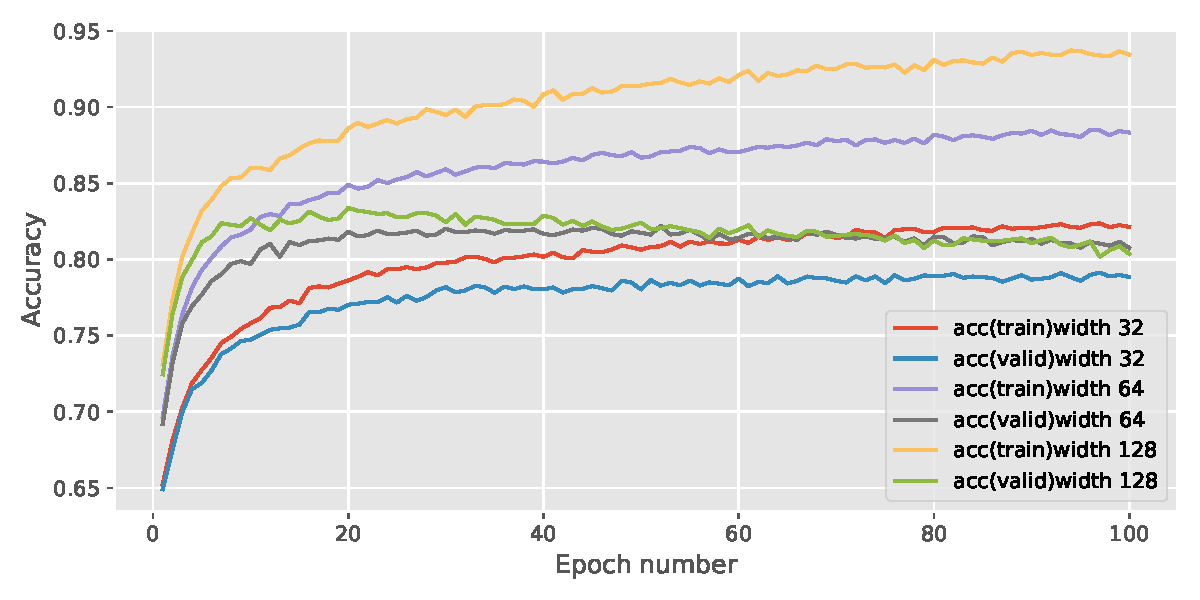
\includegraphics[width=\linewidth]{figures/one_hidden_layer_acc.pdf}
        \caption{accuracy by epoch}
        \label{fig:width_acccurves}
    \end{subfigure} 
    \begin{subfigure}{\linewidth}
        \centering
        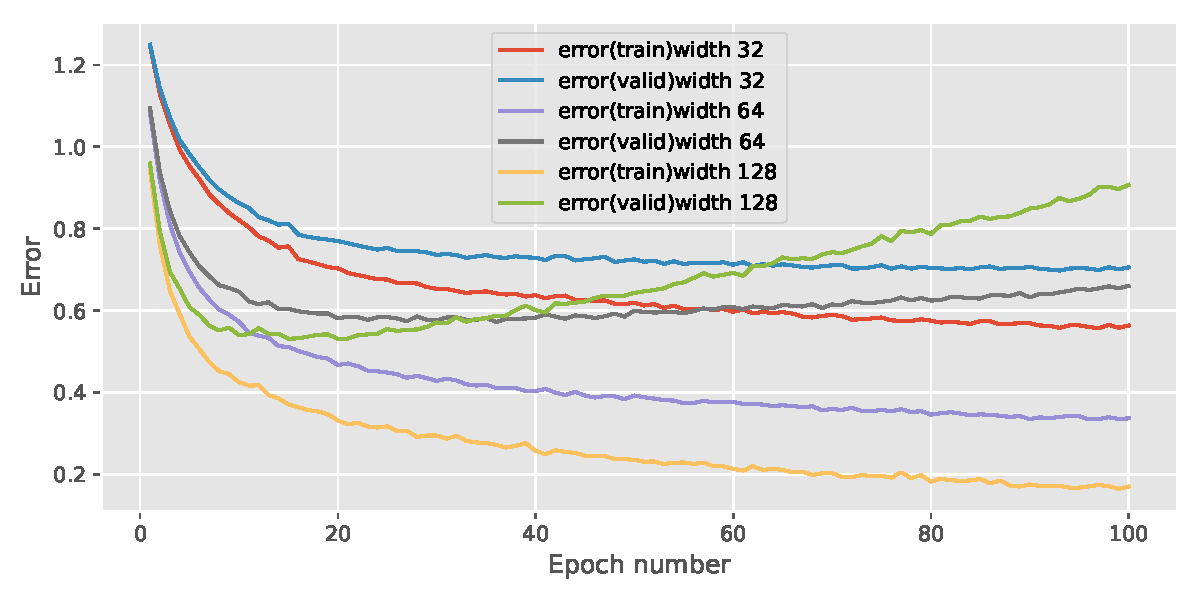
\includegraphics[width=\linewidth]{figures/one_hidden_layer_error.pdf}
        \caption{error by epoch}
        \label{fig:width_errorcurves}
    \end{subfigure} 
    \caption{Training and validation curves in terms of classification accuracy (a) and cross-entropy error (b) on the EMNIST dataset for different network widths.}
    \label{fig:width}
\end{figure} 
}
}

%% Question Figure 3:
\newcommand{\questionFigureThree} {
\youranswer{Question Figure 3 - Replace these images with figures depicting the accuracy and error, training and validation curves for your experiments varying the number of hidden layers.
%
\begin{figure}[t]
    \centering
    \begin{subfigure}{\linewidth}
        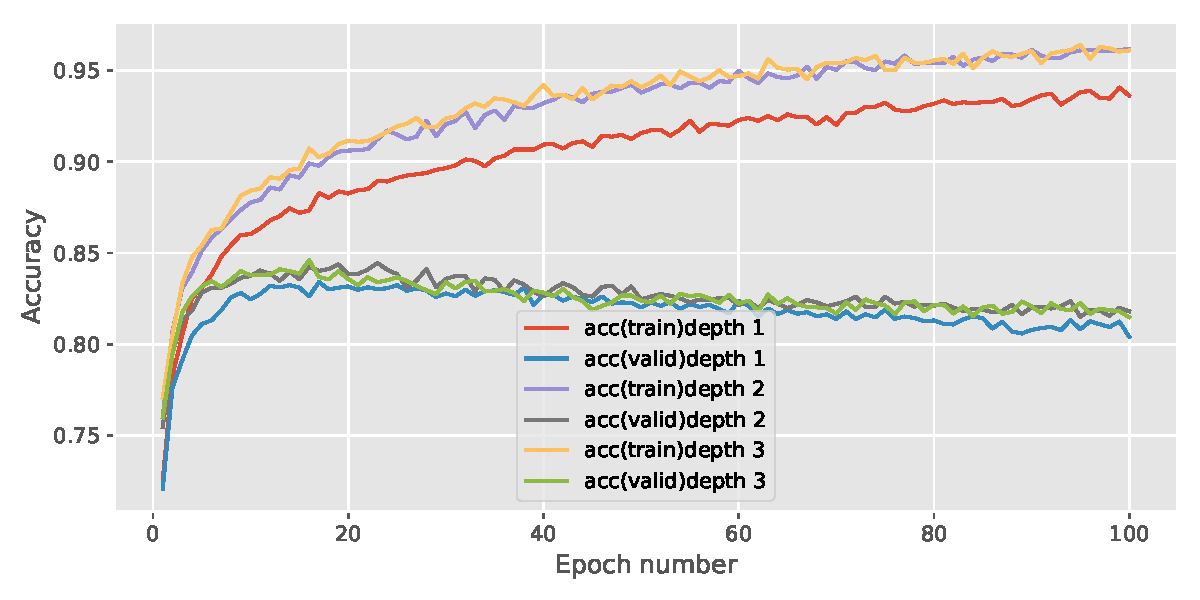
\includegraphics[width=\linewidth]{figures/multiple_layers_acc.pdf}
        \caption{accuracy by epoch}
        \label{fig:depth_acccurves}
    \end{subfigure} 
    \begin{subfigure}{\linewidth}
        \centering
        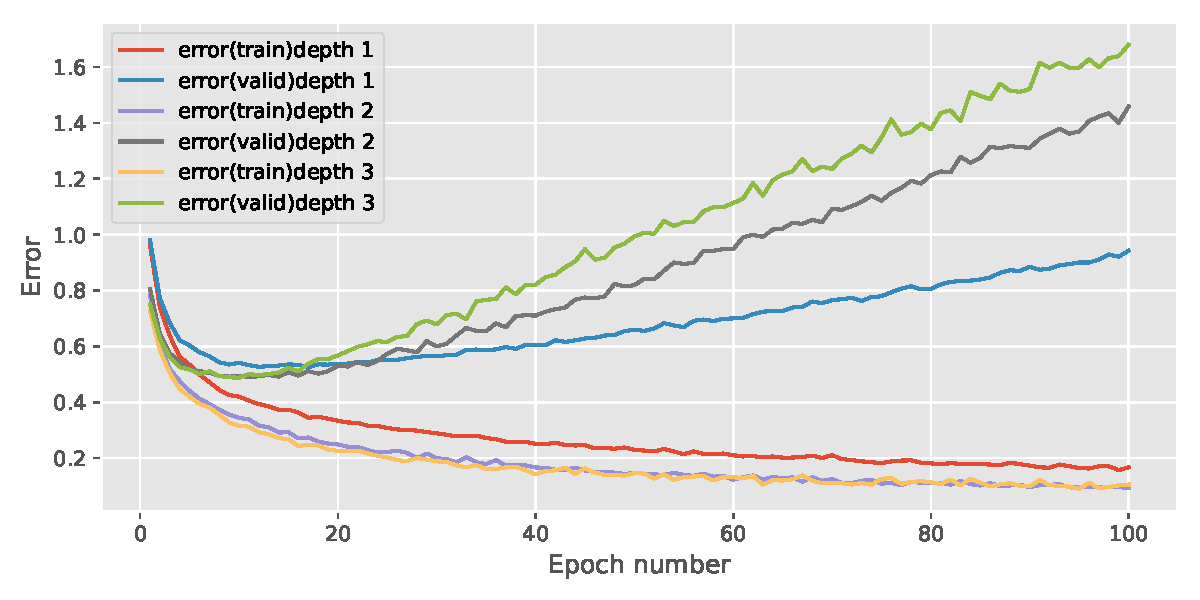
\includegraphics[width=\linewidth]{figures/multiple_layers_error.pdf}
        \caption{error by epoch}
        \label{fig:depth_errorcurves}
    \end{subfigure} 
    \caption{Training and validation curves in terms of classification accuracy (a) and cross-entropy error (b) on the EMNIST dataset for different network depths.}
    \label{fig:depth}
\end{figure} 
}
}

%% Question Figure 4:
\newcommand{\questionFigureFour} {
\youranswer{Question Figure 4 - Replace these images with figures depicting the Validation Accuracy and Generalisation Gap (difference between validation and training error) for each of the experiment results varying the Dropout inclusion rate, and L1/L2 weight penalty depicted in Figure 3 (including any results you have filled in).
%
\begin{figure*}[t]
    \centering
    \begin{subfigure}{.475\linewidth}
        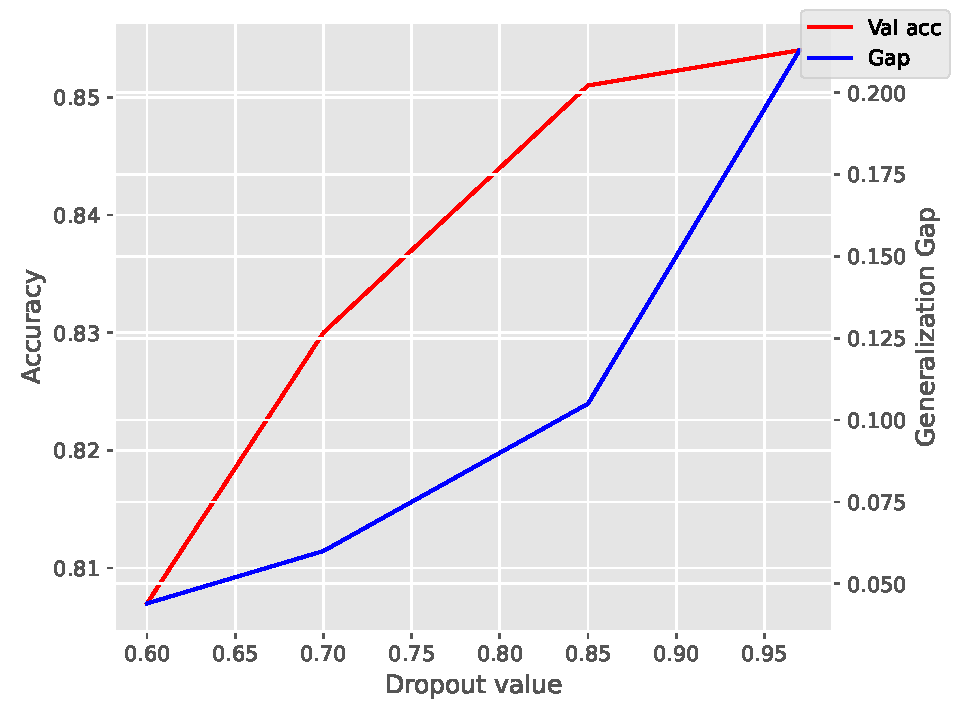
\includegraphics[width=\linewidth]{figures/Dropout_value.pdf}
        \caption{Accuracy and error by inclusion probability.}
        \label{fig:dropoutrates}
    \end{subfigure} 
    \begin{subfigure}{.475\linewidth}
        \centering
        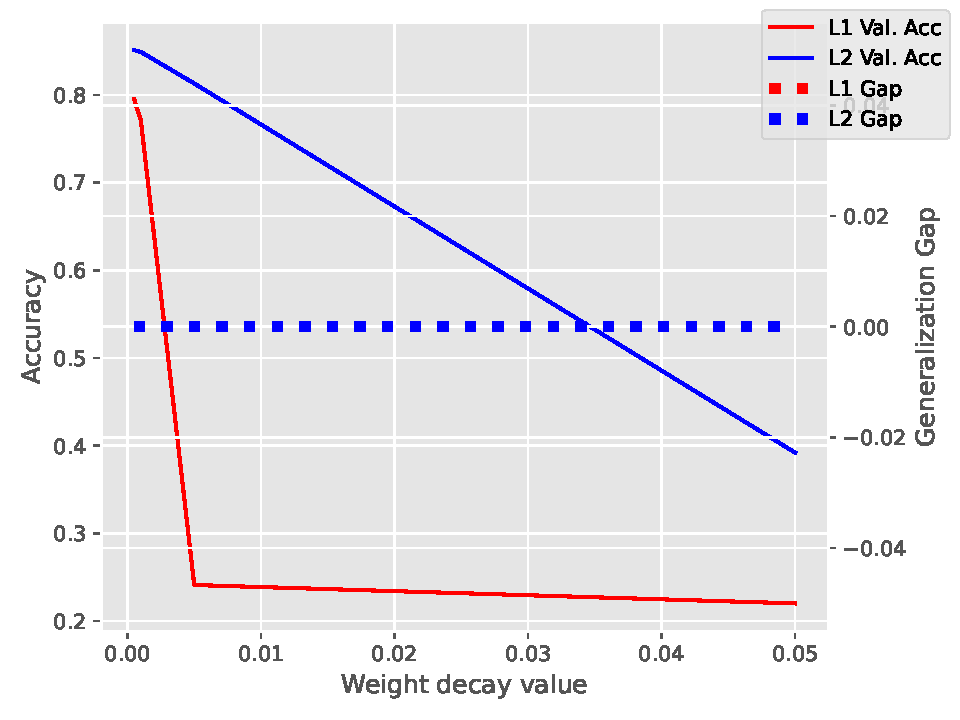
\includegraphics[width=\linewidth]{figures/weight_decay.pdf}
        \caption{Accuracy and error by weight penalty.}
        \label{fig:weightrates}
    \end{subfigure} 
    \caption{Accuracy and error by regularization strength of each method (Dropout and L1/L2 Regularization).}
    \label{fig:hp_search}
\end{figure*}
}
}

%% - - - - - - - - - - - - TABLES - - - - - - - - - - - - 

%% Question Table 1:
\newcommand{\questionTableOne} {
\youranswer{
Question Table 1 - Fill in Table 1 with the results from your experiments varying the number of hidden units.
%
\begin{table}[t]
    \centering
    \begin{tabular}{c|ccc}
    \toprule
        \# Hidden Units & Val. Acc. & Train Error & Val. Error\\
    \midrule
         32            &    78.9   &  0.563 &   0.705            \\
         64            &    80.8   &  0.337  &   0.660            \\
         128           &    80.4   &  0.170  &   0.907           \\ 
    \bottomrule
    \end{tabular}
    \caption{Validation accuracy (\%) and training/validation error (in terms of cross-entropy error) for varying network widths on the EMNIST dataset.}
    \label{tab:width_exp}
\end{table}
}
}

%% Question Table 2:
\newcommand{\questionTableTwo} {
\youranswer{
Question Table 2 - Fill in Table 2 with the results from your experiments varying the number of hidden layers.
%
\begin{table}[t]
    \centering
    \begin{tabular}{c|ccc}
    \toprule
        \# Hidden Layers & Val. Acc. & Train Error & Val. Error \\
    \midrule
         1               &     80.4       &  0.167   &       0.942          \\
         2               &    81.8       &  0.0925 & 1.46                 \\
         3               &      81.5      &   0.105 & 1.68               \\ 
    \bottomrule
    \end{tabular}
    \caption{Validation accuracy (\%) and training/validation error (in terms of cross-entropy error) for varying network depths on the EMNIST dataset.}
    \label{tab:depth_exps}
\end{table}
}
}

%% Question Table 3:
\newcommand{\questionTableThree} {
\youranswer{
Question Table 3 - Fill in Table 3 with the results from your experiments for the missing hyperparameter values for each of L1 regularisation, L2 regularisation, and Dropout (use the values shown on the table).
%
\begin{table*}[t]
    \centering
    \begin{tabular}{c|c|ccc}
    \toprule
        Model    &  Hyperparameter value(s) & Validation accuracy & Train Error & Validation Error \\
    \midrule
    \midrule
        Baseline &  -                    &               83.7 &       0.241 &  0.533          \\
    \midrule
        \multirow{4}*{Dropout}
                 & 0.6                   &  80.7                &      0.549 & 0.593     \\
                 & 0.7 & 83.0 & 0.442 & 0.502  \\
                 & 0.85 & 85.1 &  0.329 &  0.434 \\
                 & 0.97 & \textbf{85.4} &  0.244 & 0.457  \\
    \midrule
        \multirow{4}*{L1 penalty}
                 & 5e-4 & \textit{79.5} & 0.642 & 0.658 \\
                 & 1e-3 & 77.1 & 0.744 & 0.764 \\
                 & 5e-3 & 2.41 & 3.850 & 3.850 \\
                 & 5e-2 & 2.20 & 3.850 & 3.850 \\
    \midrule
        \multirow{4}*{L2 penalty}  
                 & 5e-4 & \textit{85.1} & 0.306 & 0.460 \\
                 & 1e-3 & 84.9 & 0.334 & 0.450 \\
                 & 5e-3 & 81.3 & 0.586 & 0.607 \\
                 & 5e-2 & 39.2 & 2.258 & 2.256  \\      
    \bottomrule
    \end{tabular}
    \caption{Results of all hyperparameter search experiments. \emph{italics} indicate the best results per series (Dropout, L1 Regularization, L2 Regularization) and \textbf{bold} indicates the best overall.}
    \label{tab:hp_search}
\end{table*}
}
}

%% END of YOUR ANSWERS